\section{Re- conception de l'ACV} 
\subsection{FAST}
\label{subsec:FAST}
Nous soulignons au sein de ces diagrammes FAST les pistes suivies par un astérisque.
Nous ne présentons que les premières pour souligner la production de redondances pour la compréhension de la construction de la figure~\ref{fig:FAST_remix}.
%\colorbox{yellow}{restreindre le nombre de fonctions traitées par FAST montrant une redondance.}

\resizebox{0.75\textwidth}{!}{
\begin{minipage}{\textwidth} 

%\begin{landscape}
\footnotesize

\begin{fast}{FS1 \\ Présenter la préférence du décideur sur des alternatives.}
	\FT{FT11 Décrire des systèmes d'objets}{
		\FT{FT111 Employer des langages de description}{
			\FT{}{
%				\ST{ST1111 UML}
				\ST{ST1111 RDFS}
				}
			\FT[ou]{}{
				\ST{ST1112 SKOS}
				}
			\FT[ou]{}{
				\ST{ST1113 OWL}
			}
		}
	}
	\FT{FT12 Décrire des systèmes de valeurs}{
		\FT{FT121 Décrire les dimensions du système}{
			\FT{FT111}{}
		}
		\FT{FT122 Définir les rapports entre dimensions}{
			\FT{FT1221 Employer une méthode d'agrégation partielle}{
				\ST{ST12211 ELECTRE}
				\ST[ou]{ST12212 PROMETHEE \cite{deshmukh_preference_2013}}
			}
			\FT[ou]{FT1222 Employer une méthode d'agrégation complète*}{
				\ST{ST12221 AHP* / ANP \cite{saaty_decision_2004, saaty_fundamentals_2004}}
			}
		}
	}
	\FT{FT13 Assurer la consistance du jugement}{
		\FT{FT131 Contrôler la consistance du jugement}{
			\FT{}{
				\ST{Ratio d'inconsistance (RI)}
				}
			\FT{}{
				\ST{Consistence et erreur relative \cite{barzilai_consistency_1998}}
				}
			}
%		}
		\FT{FT132 Exploiter des fractions consistantes}{
			\FT{FT1321 Permettre l'emploi de systèmes partiels}{
				\ST{Normalisation local du système de valeur}
			}
			\FT[ou]{FT1322 Extraire la composante consistante}{
				\ST{Décomposition matricielle \cite{barzilai_consistency_1998}}
			}
		}
	}
	\FT{FT15 Appliquer des valeurs aux descriptions d'objets}{
		\FT{FT151 Interroger les descriptions de systèmes}{
			\FT{FT1511 Employer un  language de requête}{
				\ST{SPARQL \cite{harris_sparql_2013}}
			}
		}
	}
		\FT{FT152 Appliquer le jugement par un MCDM}{
			\FT{FT1511 Surclassement flou}{
				\ST{ST15111 = ST12211}
				\ST[ou]{ST15112 = ST12212}
			}
		}
%	}
\end{fast}
\fastReset
\end{minipage}
}
\figbox{Au sein même d'une fonction de service, des solutions techniques identiques répondent à plusieurs fonctions techniques.
Elles sont alors reprise par leur désignation alphanumérique, telle par exemple la FT111.}
\resizebox{0.75\textwidth}{!}{
\begin{minipage}{\textwidth} 

\footnotesize
\begin{fast}{FS2\\ Respecter les limites cognitives humaines.}

\FT{FT21 Décomposer les tâches sous les niveaux de surcharge cognitive.}{
\FT{FT211 Limiter ne nombre d'objet à mémoriser}{
\FT{FT2111 Employer un support}{
\ST{ST21111 Ordinateur}
}
}
\FT{FT1X}{}
%\FT{FT11}{\FASTVide{...}}
%\FT{FT12}{\FASTVide{...}}
%\FT{FT13}{\FASTVide{...}}
}
\end{fast}
\fastReset
\end{minipage}
}
\figbox{La FS2 est quasi caricaturale de l'interconnexion des problèmes à résoudre et de l'unicité de la résolution technique.
La totalité de l'aval (traitement du "comment ?") est commune à FS1.
Hors des FT1x et donc des ST1x, l'ordinateur ST21111, en tant qu'outil universel est tacite à l'ensemble des solutions informatiques.}

Allégeons un peu le formalisme pour présenter encore un FAST.

\resizebox{0.85\textwidth}{!}{
\begin{minipage}{\textwidth}
\footnotesize
\begin{fast}{FS3\\ Être adaptée aux distributions culturels.}
\FT{FT31 Être lisible, éditable, utilisable partout sur le globe}{
	\ST{ST311 = ST21111 Ordinateur}
	\ST{ST312 Web2.0}
	\FT{FT111}{}
%	\FT{}{}
		}
\FT{FT32 Permettre l'emploi d'ontologies multiples}{
	\FT{FT111}{}
	}
\FT{FT33 Permettre un compréhension mutuelle}{
		\FT{FT331 Employer des normes internationales}{
		\ST{ST3311 W3C*(ST1111-3 ; ST312)}}
		}
\end{fast}
\fastReset
\end{minipage}
}
\figbox{Sur FS3, l'évolution majeure d'un support de communication globale recouvre le graphe comme il recouvre la planète et le multiples activités qu'elle compte en elle.}

%\resizebox{0.85\textwidth}{!}{
%\begin{minipage}{\textwidth} 
%\begin{fast}{FS4\\ Assurer son développement en données.}
%\FT{FT41 Permettre au plus grand nombre de personnes de contrôler - éditer des données}{
%	\FT{FT411 = FT31
%	%Être lisible, éditable, réalisable librement partout sur le globe
%	}{}
%	}
%\FT{FT42 Étendre la communauté d'utilisateur - contributeur}{
%	\FT{FT421 Favoriser l'usage}{
%		\FT{FT411}{}
%		}
%	\FT{FT422 Favoriser la contribution}{}
%	}
%\FT{FT43 Permettre la communication des différentes disciplines scientifiques (cultures).}{
%	\FT{FT32}{}
%	\FT{FT33}{
%		\FT{FT331}{}
%		}
%	}
%\FT{FT44 Permettre la production par programme informatique}{
%	\FT{FT441 Permettre la lisibilité - requêtabilité machine}{}
%	}
%\end{fast}
%\fastReset
%\end{minipage}
%}
%
%\resizebox{0.85\textwidth}{!}{
%\begin{minipage}{\textwidth} 
%\begin{fast}{FS5 Être valide et crédible.}
%\FT{Assurer la correction des données}{}
%\FT{Assurer un contrôle expert}{
%	\FT{Permettre le contrôle de l'expertise de l'éditeur}{
%		\FT{Déclarer nominativement et en responsabilité les descriptions}{}
%		}
%	\FT{Réaliser une revue par les pairs}{
%	\ST{}
%	}
%	}
%\FT{Assurer la responsabilité des auteurs}{
%	\FT{Déclarer nominativement et en responsabilité les descriptions}{}
%	}
%\FT{Faciliter la curation}{}
%\FT{Permettre à un grand nombre de personne de contrôler - éditer un grand nombre de données}{}
%\FT{Faciliter la production des descriptions d'objets}{}
%\FT{Faciliter la production des déclarations de valeurs}{}
%\FT{Site interactif}{}
%\FT{Système de gestion de version transparent et sécurisé}{}
%\end{fast}
%\fastReset
%\end{minipage}
%}
%
%\resizebox{0.85\textwidth}{!}{
%\begin{minipage}{\textwidth} 
%\begin{fast}{FS6 Respecter les contraintes réglementaires.}
%\FT{Éviter les objets protégés}{}
%\FT{S'assurer un large soutien de la société civile}{}
%\end{fast}
%\fastReset
%\end{minipage}
%}
%
%\resizebox{0.85\textwidth}{!}{
%\begin{minipage}{\textwidth} 
%\begin{fast}{FS7 Protéger les déclarants sur l’énoncé de leurs jugements.}
%\FT{non exploré}{}
%\end{fast}
%\fastReset
%\end{minipage}
%}
%
%%\end{landscape}
%\colorbox{yellow}{Voir Help p21 pour les solutions techniques à plusieurs fonctions}
%\colorbox{yellow}{http://sciences-indus-cpge.papanicola.info/Diagramme-FAST-avec-Tikz-et-Latex}
%
%\begin{center}
%\colorbox{red}{fin - ANNEXES}
%\end{center}

\subsection{Un nouveau standard}
\label{sec:Un nouveau standard}
Comme indiqué au \ref{sec:Re-conception de l'ACV, conclusion et perspective} et au \ref{sec:Conclusion sur la multifonctionnalité}, la nécessaire évolution des normes doit comprendre l'intégration du jugement morale.
\figbox{Sur la figure~\ref{fig:ILCD-V2}, nous pouvons observer l'extension nécessaire du cadre de travail de l'évaluation en cycle de vie.
Cette représentation fait apparaître la volonté de démarcation entre but et périmètre entre le cadre de travail de l'ISO et de l'ILCD.
Nous poursuivons la modification de ce cadre avec l'intégration d'une étape de déclaration explicite du jugement du décideur.
Nous signalons également la nécessité de l'emploi des techniques d'\gls{ADMC} pour l'interprétation.}
\begin{figure}[htbp]
\centering
  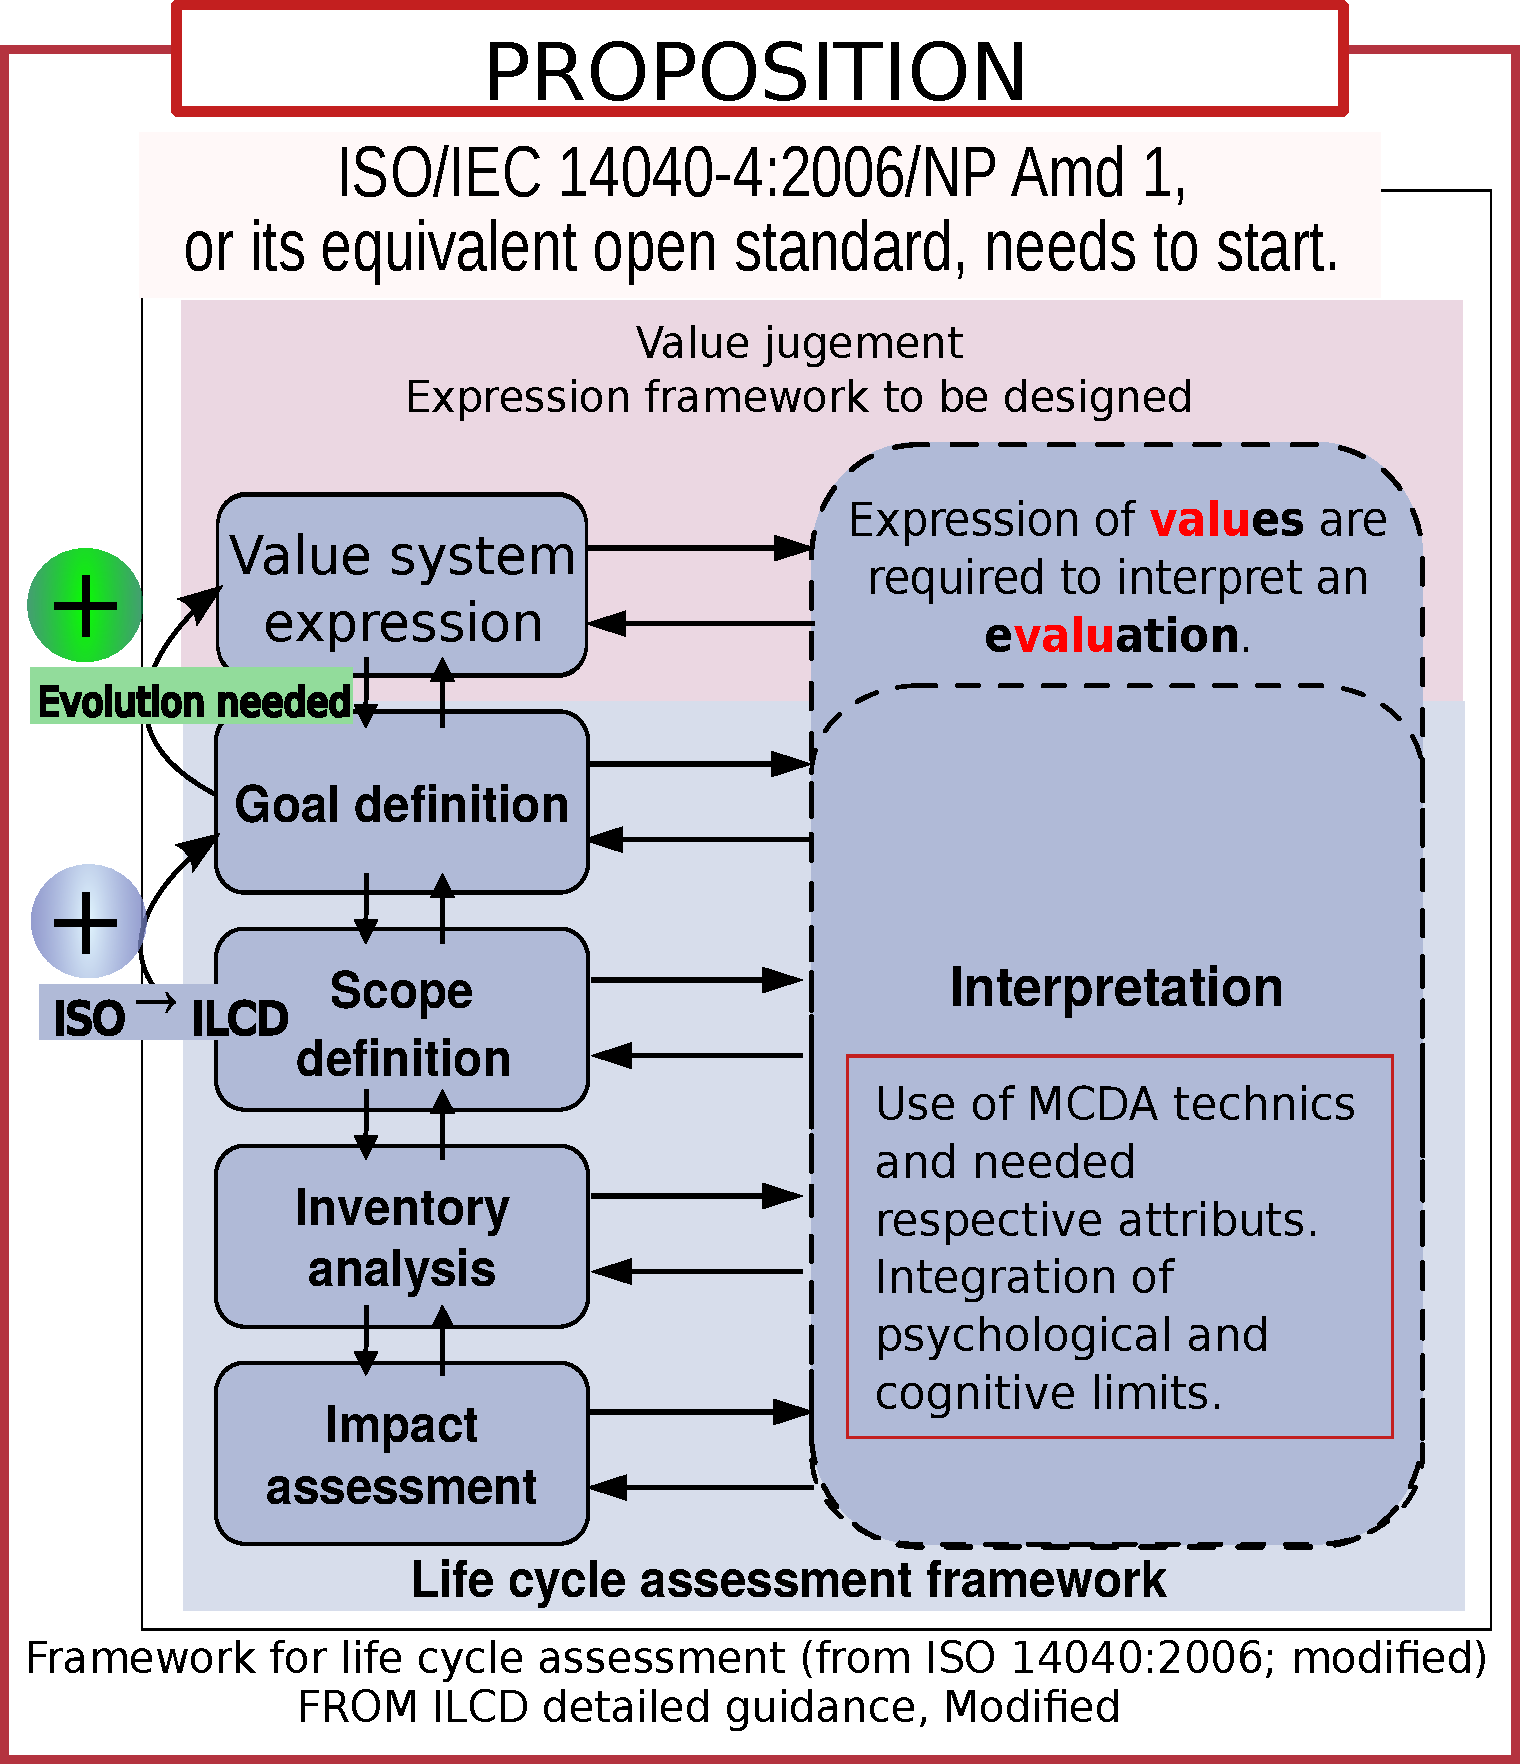
\includegraphics[width=0.8\textwidth]{/home/rudy/Documents/rudy/01_These/11_production/01_COMMUNICATION/figures/proposition_ILCD-V2.pdf}
  \caption{Proposition de révision de l'ISO~14040 et l'ILCD. Extrait~\cite{patard_life_2015}.}
  \label{fig:ILCD-V2}
\end{figure}
